\section{Additional experiments and audits}

\subsection{Synthetic, comparator, and runtime experiments}
\IfFileExists{generated/results_table.tex}{\begin{table}[H]
\centering
\caption{Mean baseline MSE over 100 preregistered trials. Oracle labels indicate per-signal ground-truth tuning.}
\label{tab:synthetic}
\begin{tabular}{lrrr}
\toprule
Method & Exact, $\sigma=0$ & Exact, $\sigma=0.1$ & Variable, $\sigma=0.1$ \\
\midrule
Centred HCRD & 0 & 0.787 & 0.887 \\
Thresholded HCRD & 3.78e-32 & 0.00778 & 0.312 \\
Adaptive guided HCRD & 0.0124 & 0.0385 & 0.0856 \\
Gaussian oracle & 0.0433 & 0.0382 & 0.0632 \\
Moving-average oracle & 0.0516 & 0.0486 & 0.0743 \\
\bottomrule
\end{tabular}
\end{table}
}{}

As a computational audit rather than a proof, we also simulated 50,000 null
and alternative draws for a fixed 24-template compact-lobe dictionary in 257
samples.  Its maximum coherence was 0.0376.  At the conservative theorem
threshold for $\alpha=0.05$, empirical false rejection was 0.00524 (Wilson
interval $[0.00464,0.00591]$).  At the sufficient power norm, miss probability
was 0.0363 versus the guaranteed bound 0.20; at the localisation norm, no error
was observed (upper Wilson limit $7.68\times10^{-5}$) versus the bound 0.10.
These checks expose conservatism and implementation errors; they do not replace
Theorem~\ref{thm:lobe-scan}.

We separately audited Theorem~\ref{thm:continuous-scan} on 129 samples and a
595-template centre--width--asymmetry sieve.  In 50,000 null draws the finite
threshold 4.332 was exceeded 22 times: empirical FWER 0.00044 with 95\%
Wilson interval $[0.000276,0.000666]$.  Its true-template Gaussian sufficient norm
5.1739 for $\beta=0.2$ gave empirical power 0.8773 in 10,000 draws.  For the
complete continuum, $q=127$: the projected-norm envelope threshold 12.4218
was exceeded in 2537/50,000 direct projected-norm draws, giving 0.05074
($[0.04883,0.05270]$), while the closed-form Laurent--Massart threshold
13.1150 was exceeded with probability 0.00486.  The resulting conservative
80\%-power sufficient norm is 13.2634.  This replaces the earlier Dudley
sufficient norm 285.1103 without treating the numerical grid as the continuum.
These draws audit the dominating norm, not the generally smaller scan null.
The finite sieve remains sharper because it declares only 595 templates rather
than the full residual subspace.

On 100 fresh noiseless exact-class trials, centred HCRD recovered the latent
baseline to numerical zero.  It had lower MSE in every trial than the historical
legacy rule and the oracle-tuned Gaussian, moving-average, and Fourier
comparators.  All corresponding paired bootstrap intervals were below zero and
Holm-adjusted sign-test values were below $1.6\times10^{-29}$.  Thresholded HCRD
and an endpoint-only RDP baseline were also exact within $10^{-12}$ and are
reported as ties, not losses.  That RDP solution uses only the two domain
endpoints: it recovers the global affine baseline but not the $J-1$ lobe
boundaries, so it does not tie the boundary-recovery endpoint in
Figure~\ref{M-fig:recovery-phase}.  On the exploratory variable-amplitude,
piecewise-affine class without noise, centred HCRD had mean MSE $0.0179$, versus
$0.0645$ for the Gaussian oracle, but the raw method failed under sample-level
white noise.  Adaptive guidance improved knot accuracy substantially; its
pilot-calibrated scale is not yet supported by a distribution-free theorem.

An external-method experiment then used 50 further exact-class trials.  On the
noiseless condition, centred HCRD had lower baseline MSE in all 50 trials than
the final EMD residue, the lowest-frequency VMD mode, and per-signal
oracle-tuned $\ell_1$ trend filtering.  The respective mean competitor MSEs
were $0.0108$, $0.511$, and $0.0425$, versus zero for HCRD; every paired
bootstrap interval was below zero and the Holm-adjusted sign-test value was
$1.07\times10^{-14}$.  A supplementary direct comparison on the same 50 fixed
draws used the final ITD baseline returned by PySDKit 0.4.54.  ITD mean MSE was
$0.1473$; the HCRD--ITD paired difference was $-0.1473$
($[-0.1871,-0.1085]$), with 50/50 HCRD wins and Holm-adjusted exact sign
$p=1.24\times10^{-14}$.  EMD, VMD, and ITD settings follow their standard
algorithms \citep{huang1998emd,dragomiretskiy2014vmd,frei2007itd}; oracle
tuning deliberately favours the smoothing comparators.  This confirmation is
specific to the chord-lobe class, rather than evidence of global dominance
over ITD's time--frequency use cases.
Although DPT is an exact nonlinear pulse decomposition, its native components
are constant pulses and do not define a unique final chord baseline at a
matched scale; it is therefore included in the structural comparison rather
than assigned an artificial baseline-MSE endpoint.

After that result, two fresh 100-trial noisy confirmations were locked on new
seeds before outcome inspection for the plug-in MAD-thresholded variant.
Table~\ref{tab:external}
reports their means.  At $\sigma=0.03$, its win rates against EMD, VMD,
$\ell_1$, and Gaussian were respectively $0.86$, $0.99$, $0.99$, and $0.98$;
at $\sigma=0.10$ they were $0.81$, $0.93$, $0.96$, and $0.74$.  All paired
bootstrap intervals remained below zero.  The largest Holm-adjusted sign-test
value was $1.67\times10^{-6}$.  This finite-sample confirmation concerns the
specified generator and plug-in estimator; Theorem~\ref{M-thm:noise} itself assumes known or
externally estimated noise scale.

\begin{table}[H]
\centering
\caption{Mean baseline MSE for external comparisons.  The noiseless column is
E1 (50 trials); noisy columns are fresh C2 confirmations (100 trials each).}
\label{tab:external}
\begin{tabular}{lrrr}
\toprule
Method & $\sigma=0$ & $\sigma=0.03$ & $\sigma=0.10$ \\
\midrule
Centred HCRD & 0 & 0.762 & 0.789 \\
Thresholded HCRD & $2.92\times10^{-32}$ & 0.00356 & 0.0195 \\
EMD residue & 0.0108 & 0.0288 & 0.0531 \\
VMD low mode & 0.511 & 0.0344 & 0.0396 \\
$\ell_1$ trend oracle & 0.0425 & 0.0419 & 0.0443 \\
Gaussian oracle & 0.0378 & 0.0336 & 0.0383 \\
\bottomrule
\end{tabular}
\end{table}

Two additional external decompositions were then tested under independently
frozen, fresh-seed protocols.  Improved complete ensemble EMD with adaptive
noise (CEEMDAN) \citep{colominas2014ceemdan} used 20 noise realizations and an
oracle selected, separately for every signal, the cumulative one-to-four
slowest components that minimized latent-baseline MSE.  Fast Iterative
Filtering used the author-linked Python implementation with its published
defaults \citep{cicone2021fif}.  Its oracle used the analogous cumulative
slow-tail selection.  Both oracles use unavailable ground truth and therefore
favour the comparators.

Table~\ref{tab:modern-decomposition} reports the results.  In E2, HCRD won
50/50, 48/50, and 35/50 paired trials at noise standard deviations 0, 0.03,
and 0.10; the largest Holm-adjusted sign-test value was 0.00660, and all three
95\% bootstrap intervals for HCRD minus CEEMDAN lay below zero.  In E3 the
corresponding wins over oracle Iterative Filtering were 50/50, 50/50, and
49/50, with largest adjusted value $9.06\times10^{-14}$ and again all
intervals below zero.  These confirmations strengthen only the stated
chord-lobe baseline task: CEEMDAN and Iterative Filtering target oscillatory
mode decompositions rather than endpoint-chord recovery.

\begin{table}[H]
\centering
\caption{Fresh modern-decomposition confirmations (50 signals per condition).
The HCRD reference is centred at $\sigma=0$ and MAD-thresholded otherwise.
E2 and E3 use independent seeds and must be read as paired rows within study.}
\label{tab:modern-decomposition}
\begin{tabular}{llrrr}
\toprule
Study & Method & $\sigma=0$ & $\sigma=0.03$ & $\sigma=0.10$ \\
\midrule
E2 & HCRD reference & 0 & 0.000400 & 0.00636 \\
E2 & CEEMDAN oracle slow tail & 0.0135 & 0.0137 & 0.0312 \\
\addlinespace
E3 & HCRD reference & 0 & 0.000398 & 0.0124 \\
E3 & Iterative Filtering oracle tail & 0.135 & 0.156 & 0.143 \\
\bottomrule
\end{tabular}
\end{table}

Finally, an exploratory Case Western Reserve University bearing study used
12~kHz drive-end recordings for four states and four motor loads
\citep{smith2015cwru}.  Complete recordings, rather than randomly mixed
windows, defined leave-one-load-out folds.  Raw summary features already
reached mean balanced accuracy $0.982$; Gaussian, wavelet, EMD, and raw HCRD
representations all reached $1.000$.  Thus the data exhibit a ceiling effect
and provide no evidence that HCRD is superior.  Guided HCRD was worse at
$0.945$, including $0.781$ on the 3-hp fold.  The experiment therefore
identifies a ceiling regime in which HCRD provides no classification benefit.

Runtime protocol P1 processed the same 384 CWRU windows five times per mode in
randomized order after a whole-system load gate; compiled-library thread counts
were fixed to one, and pool startup and serialization were timed. Every one of
the 35 feature
matrices was bitwise identical to the saved R1 matrix.  On an Intel Core Ultra
7 155H, serial median latency was 10.279 s.  Two, four, eight, and sixteen
worker processes achieved respectively 1.76, 2.16, 2.47, and 2.00 times
speedup; four and eight Python threads achieved only 0.55 and 0.60 times serial
performance because the reference knot walk is GIL-bound. The complete
machine-specific scaling results are provided in the repository. Levels
within one signal remain
sequential, whereas independent windows, records, and channels are exactly
parallel.

We implemented Corollary~\ref{M-cor:sparse} by storing only nested knot sets and
materializing dense arrays on demand. Protocol P2R required five consecutive
one-second whole-system samples, each at most 20\%, before every trial.  Every
timed hierarchy had the same canonical knot digest, and materialized features
for all 384 windows were bitwise identical to R1.  Sparse serial construction
reduced the median from 14.461 to 1.217 s, an 11.89-fold representation-level
speedup; four processes further reduced it to 0.976 s (1.25-fold versus sparse
serial).  Eight processes did not amortize startup and serialization on this
short batch.

Protocol P3 therefore froze a tenfold larger 3840-window throughput batch under
the same per-trial load gate.  Table~\ref{tab:sparse-runtime} shows monotone
process scaling to a 1.96-fold end-to-end speedup with eight workers.  This
supports exact independent-signal parallelism, but not ideal linear scaling;
all timings include pool construction, serialization, output collection, and
hierarchy allocation.

\begin{table}[H]
\centering
\caption{Strictly load-gated sparse runtime results.  Speedup is relative to
dense serial in P2R and sparse serial in P3.}
\label{tab:sparse-runtime}
\begin{tabular}{llrrrr}
\toprule
Protocol & Representation/backend & Workers & Signals & Median (s) & Speedup \\
\midrule
P2R & dense serial & 1 & 384 & 14.461 & 1.00 \\
P2R & sparse serial & 1 & 384 & 1.217 & 11.89 \\
P2R & sparse process & 4 & 384 & 0.976 & 14.82 \\
P3 & sparse serial & 1 & 3840 & 13.682 & 1.00 \\
P3 & sparse process & 2 & 3840 & 11.911 & 1.15 \\
P3 & sparse process & 4 & 3840 & 8.669 & 1.58 \\
P3 & sparse process & 8 & 3840 & 6.963 & 1.96 \\
\bottomrule
\end{tabular}
\end{table}

A separate new-seed confirmation assessed the quadratic proximal guide with a
single pilot-selected but then frozen value $\lambda=3$ on the variable-amplitude
chord-lobe generator.  Thirty independent latent signals, each with ten noise
repetitions, were used at every noise level; inference averaged repetitions
within latent signal.  Table~\ref{tab:stable} shows a morphology advantage.
Against the adaptive Gaussian guide, paired F1 differences were $0.274$, $0.244$,
and $0.191$ for $\sigma=0.01,0.03,0.05$, with all 95\% bootstrap intervals
strictly positive; at $\sigma=0.10$ the difference was $0.011$ with interval
$[-0.015,0.039]$, an explicit tie.  Quadratic guidance also exceeded raw,
thresholded, and fixed-Gaussian HCRD at every noise level after Holm correction.
The maximum sampled guide perturbation ratio was $0.366$, consistent with
Theorem~\ref{M-thm:prox}; after hard HCRD it reached $2.543$, confirming that the
global theorem must not be transferred to the knot output.

\begin{table}[H]
\centering
\caption{Frozen S2 confirmation.  F1 matches latent chord knots within one
sample.  MSE is against the latent baseline.}
\label{tab:stable}
\begin{tabular}{rrrrrr}
\toprule
$\sigma$ & Quad. F1 & Adaptive F1 & Fixed-Gauss. F1 & Quad. MSE & Adaptive MSE \\
\midrule
0.01 & 0.716 & 0.442 & 0.410 & 0.0730 & 0.0722 \\
0.03 & 0.720 & 0.476 & 0.399 & 0.0732 & 0.0863 \\
0.05 & 0.722 & 0.531 & 0.338 & 0.0732 & 0.0922 \\
0.10 & 0.720 & 0.709 & 0.230 & 0.0727 & 0.0964 \\
\bottomrule
\end{tabular}
\end{table}


\subsection{E2 qscore implementation sensitivity}
The main E2 comparison used a global-window independent reimplementation of
the published qscore.  We repeated both transfer directions after changing
the minimum-point rule and the across-file summaries, always comparing HCRD-8
plus a given qscore variant with that same variant alone.  Table~\ref{tab:qscore-sensitivity}
reports the complete paired analysis.

\IfFileExists{generated/qscore_sensitivity_table.tex}{\begin{table}[H]
\centering
\caption{qscore implementation sensitivity. Entries are HCRD-8 plus the indicated qscore summary minus that same qscore alone in target AP, with paired target-feature 95\% bootstrap intervals.}
\label{tab:qscore-sensitivity}
\small
\resizebox{\linewidth}{!}{%
\begin{tabular}{lrcc}
\toprule
Variant & Width & Falkor $\to$ MESOSCOPE & MESOSCOPE $\to$ Falkor \\
\midrule
Current median, $m\geq8$ & 2 & 0.1181 [0.0628, 0.1769] & 0.1005 [0.0554, 0.1457] \\
Median, $m\geq5$ & 2 & 0.1244 [0.0688, 0.1832] & 0.0987 [0.0538, 0.1432] \\
Author-like five-summary, $m\geq5$ & 5 & 0.1517 [0.0813, 0.2184] & 0.0765 [0.0324, 0.1211] \\
Multisummary seven-variable, $m\geq8$ & 7 & 0.0847 [0.0320, 0.1407] & 0.0798 [0.0347, 0.1262] \\
\bottomrule
\end{tabular}
}
\end{table}
}{}

\subsection{Expert-labelled chromatographic lobes}
We evaluate HCRD for LC--MS peak-shape curation. A genuine extracted-ion
chromatogram (EIC) is approximately a compact, predominantly one-sign lobe over
a local baseline, whereas shoulders, split peaks, baseline fragments, and noise
violate that structure.  The public data of \citet{muller2020eic} contain
255,000 EICs: 5000 candidate ions evaluated in each of 51 real samples by mass-
spectrometry experts.  Before reading the arrays or classification table, we
froze a double group holdout.  Sample identifiers and candidate-ion identifiers
were hashed independently; a case was admitted only when both hashes assigned
it to the same train, validation, or confirmation block.  Confirmation thus
shared neither samples nor candidate ions with model development.

Every representation received both time windows shown to the experts.  The
same fixed histogram-gradient-boosted classifier was trained on robustly
resampled raw EICs, a conventional multiscale morphology bank, raw plus one
HCRD level, raw plus the complete eight-level HCRD hierarchy, HCRD scalar
geometry without waveform channels, or polygon-area/energy summaries alone.
Validation selected the conventional domain bank before the confirmation block
was unlocked.  Primary inference used a 10,000-replicate two-way cluster
bootstrap over both held-out samples and held-out candidate ions.

Table~\ref{tab:lcms-e1} shows the locked result.  Eight-level HCRD achieved the
largest confirmation AP, 0.4092 versus 0.3820 for the frozen comparator, and
exceeded the one-level representation by 0.0321.  The primary difference was
$0.0272$, but its cluster interval $[-0.0566,0.1010]$ crossed zero because the
double holdout left only eight independent confirmation samples.  The
pre-specified success rule therefore failed.  The ablations are nevertheless
informative: area alone was weakest, and scalar geometry without the signed
detail channels was also below the conventional comparator.  The useful object
is the complete multilevel decomposition in combination with the raw shape;
polygon mass is auxiliary rather than the method.

\begin{table}[H]
\centering
\caption{Locked E1 expert-labelled LC--MS confirmation (2692 unambiguous EICs,
297 peaks; eight sample and 706 candidate-ion groups).  AP is the primary
threshold-free endpoint.}
\label{tab:lcms-e1}
\begin{tabular}{lrrrr}
\toprule
Representation & AP & ROC AUC & MCC & Balanced acc. \\
\midrule
Raw EIC & 0.3626 & 0.8714 & 0.4150 & 0.7782 \\
Conventional domain bank & 0.3820 & 0.8801 & 0.4379 & 0.7866 \\
Raw + HCRD level 1 & 0.3771 & 0.8696 & 0.4026 & 0.7594 \\
Raw + HCRD levels 1--8 & \textbf{0.4092} & \textbf{0.8844} & \textbf{0.4418} & \textbf{0.8133} \\
HCRD scalar geometry & 0.3345 & 0.8415 & 0.3479 & 0.7409 \\
Polygon area/energy only & 0.3151 & 0.8254 & 0.3369 & 0.7451 \\
\bottomrule
\end{tabular}
\end{table}


\subsection{Application-boundary and cross-domain studies}
Two additional tests evaluated the application boundary. LCMS-E3 used the public
TargetedMSQC CSF panel and leave-one-run-out transfer across four runs
\citep{eshghi2018targetedmsqc}.  This is a deliberately morphology-saturated
setting: its 52 official variables already encode jaggedness, symmetry,
modality, width, elution shift, transition ratios, and light/heavy consistency.
On 576 eligible labelled transition pairs, QC52 AP was 0.9247 versus 0.8862
after adding the complete HCRD-8 bank.  The difference was $-0.0384$ with a
two-way run/peptide cluster interval $[-0.1455,0.0505]$, and HCRD won only one
of four held-out runs.  HCRD-8 did exceed HCRD-1, but the pre-specified test
failed.  A later compact-geometry search reached AP 0.9372 and is reported only
as development because it used these outcomes.

LCMS-E4 tested baseline recovery on 60 low-affine-deviation TIC windows from
20 raw NeatMS Dataset~1 mzML files \citep{gloaguen2022neatms}.  Single and
nested positive lobes were injected after the protocol and baselines were
scored against their known real-background target.  For nested lobes, HCRD-8
MSE was 0.1369, versus 0.1141 for per-case oracle asymmetric least squares and
0.1270 for oracle morphological opening.  It nevertheless beat HCRD-1,
Gaussian, Savitzky--Golay, and wavelet comparators on all 60 cases; the
HCRD-8--HCRD-1 mean difference was $-0.3942$ with simultaneous interval
$[-0.4082,-0.3801]$.  A post-protocol mixed-polarity analysis remained worse
than signed AsLS and symmetric morphology. Table~\ref{tab:lcms-boundaries}
summarizes these task-specific boundaries.

\begin{table}[H]
\centering
\caption{LC--MS application-boundary tests. Lower MSE is better in E4.}
\label{tab:lcms-boundaries}
\small
\begin{tabular}{>{\raggedright\arraybackslash}p{3.7cm}ll>{\raggedright\arraybackslash}p{4.5cm}}
\toprule
Test & HCRD & Comparator & Boundary \\
\midrule
E3 TargetedMSQC & AP 0.8862 & QC52 AP 0.9247 & morphology-saturated features \\
E4 real background & MSE 0.1369 & AsLS MSE 0.1141 & sign-aware lower envelope \\
\bottomrule
\end{tabular}
\end{table}

\subsection{Cross-domain boundary searches}
The hierarchy was also tested as a learned pulse-event representation and as a
training-free transient score. Table~\ref{tab:cross-domain-boundaries}
summarizes the results; full protocols, folds, plots, bootstrap intervals, and
ablations are provided in the repository.

\begin{table}[H]
\centering
\caption{Cross-domain boundary searches. Each row reports the corresponding
held-out or cross-fitted comparison; none is pooled with the LC--MS evidence.}
\label{tab:cross-domain-boundaries}
\small
\begin{tabular}{>{\raggedright\arraybackslash}p{2.5cm}>{\raggedright\arraybackslash}p{4.8cm}>{\raggedright\arraybackslash}p{5.5cm}}
\toprule
Test & Main result & Interpretation \\
\midrule
CWRU bearings \citep{smith2015cwru} & Raw features 0.982 balanced accuracy;
several transforms, including HCRD, tied at 1.000 & Ceiling effect; no HCRD
superiority \\
QTDB QRS \citep{laguna1997qtdb,jane1997ecgpuwave} & Quadratic HCRD 22.74 ms;
\texttt{ecgpuwave} 13.94/15.75 ms & Stable guide improves raw HCRD, but the
specialist delineator is better \\
PPG-DaLiA \citep{reiss2019ppgdalia} & Geometry F1 0.7945, mass-only 0.7659,
tuned \texttt{find\_peaks} 0.8013 & Full hierarchy carries information beyond
area, without detector superiority \\
TSB-AD/Yahoo \citep{liu2024elephant,paparrizos2022tsb} & HCRD 0.5285 AUC--PR
versus NORMA 0.3383; CNN 0.9052 & Positive frozen replication, but only within
the synthetic Yahoo family \\
Real WSD/AIOps \citep{li2022aiops} & HCRD 0.3756 versus POLY 0.4115; hybrid
0.3675 versus raw spectral residual 0.3850 & No independent real-KPI
confirmation \\
\bottomrule
\end{tabular}
\end{table}

For pulse data, the full multilevel geometry significantly exceeded the
area/energy-only ablation, confirming that polygon mass is auxiliary rather
than the decomposition.  For temporal anomaly detection we used
$S(t)=\max_{1\leq\ell\leq8}z_\ell(t)$, where $z_\ell$ is robust positive
surprise in the levelwise area-density series.  Its frozen Yahoo success did
not transfer to real WSD or AIOps KPIs and therefore does not establish general
anomaly-detection performance.


\subsection{Stability and failure-mode audits}
\begin{figure}[H]
\centering
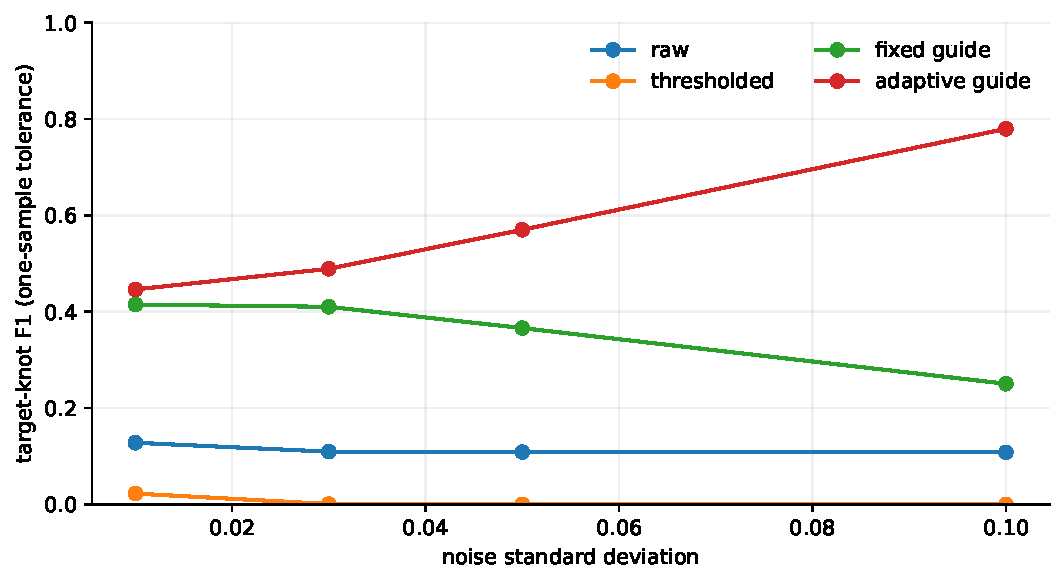
\includegraphics[width=0.92\linewidth]{figures/stability_accuracy.pdf}
\caption{Knot accuracy under repeated Gaussian perturbations.  Stability alone
is insufficient: the thresholded method is stable because it often retains
only endpoints, whereas adaptive guidance retains a compact set of meaningful
knots.}
\label{fig:stability}
\end{figure}

Theorem~\ref{M-thm:persistence} was audited on 1000 seeded perturbations, split
equally between uniform and irregular grids.  No numerical violation occurred;
the maximum observed ratio
$d_{\rm SC}/(C_x\|e\|_\infty)$ was 0.9899.  On the four-sample discontinuity
sequence, hard-baseline amplification grew from 20.5 to approximately
$2\times10^8$ as the curvature scale decreased from $10^{-1}$ to $10^{-8}$,
while the persistence distance remained exactly one half of its theorem bound
up to floating-point error (Figure~\ref{fig:persistence}).

\begin{figure}[H]
\centering
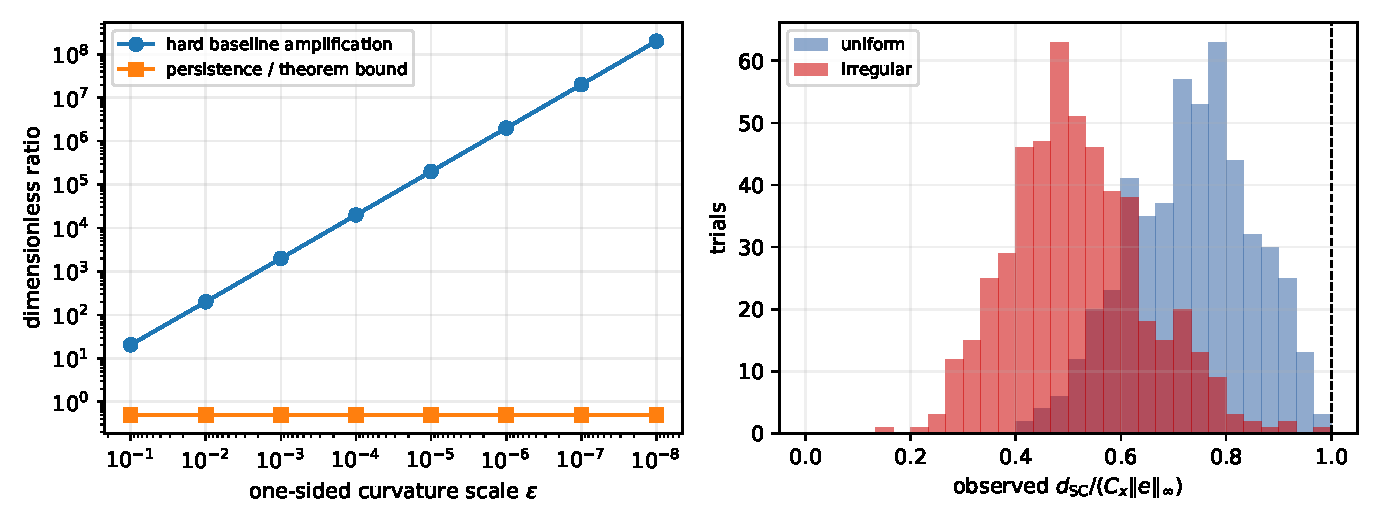
\includegraphics[width=0.96\linewidth]{figures/persistence_stability.pdf}
\caption{Hard-decision discontinuity versus signed-curvature persistence.
Left: the hard baseline has unbounded amplification while the persistence
distance remains within its global bound.  Right: all 1000 uniform/irregular-grid
checks remain below the theorem limit (dashed line).}
\label{fig:persistence}
\end{figure}
